\documentclass[10pt]{article}

\usepackage[T1]{fontenc}
\usepackage{geometry}
\usepackage{amsmath, amssymb, amsthm}
\usepackage{graphicx}
\usepackage{float}
\usepackage{multirow}
\usepackage{bm}
\usepackage{hyperref}

\geometry{a4paper, margin=1in}

\renewcommand{\labelenumi}{(\alph{enumi})}
\renewcommand{\vec}{\bm}

\DeclareMathOperator{\rank}{rank}
\DeclareMathOperator{\col}{col}

\newcommand{\C}{\mathbb{C}}
\newcommand{\R}{\mathbb{R}}
\newcommand{\Q}{\mathbb{Q}}
\newcommand{\Z}{\mathbb{Z}}
\newcommand{\N}{\mathbb{N}}

\setlength{\parindent}{0em}

\title{Assignment I}
\author{Satvik Saha}
\date{}

\begin{document}
    \noindent\textbf{IISER Kolkata} \hfill \textbf{Assignment I}
    \vspace{3pt}
    \hrule
    \vspace{3pt}
    \begin{center}
    \LARGE{\textbf{MA4206: Linear Models}}
    \end{center}
    \vspace{3pt}
    \hrule
    \vspace{3pt}
    Satvik Saha, \texttt{19MS154} \hfill \today
    \vspace{20pt}

    \setlength{\parskip}{1em}


    \section{Introduction}

    There are 90 observed abrasion resistance scores $y_{ijl}$ for jeans subjected to
    three types of denim treatments (indexed by $i$) and laundry cycles (indexed by
    $j$).

    \begin{figure}[H]
    \begin{center}
        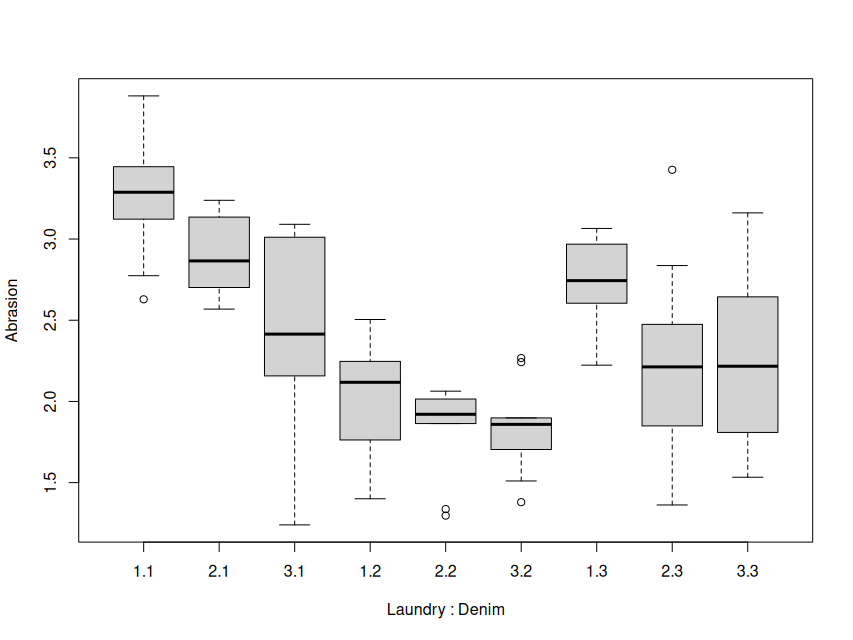
\includegraphics[width=0.9\textwidth]{boxplot.png}
    \end{center}
    \caption{
        Abrasion scores for each of the 9 groups of treatment. Lower scores are
        worse.
    }
    \label{fig:boxplot}
    \end{figure}


    These are fitted against the linear model \[
        y_{ijl} = \mu + \tau_i + \beta_j + \epsilon_{ijl}.
    \] By collecting the observations $y_{ijl}$ into a vector $\vec{y}_{90\times 1}$,
    our model looks like \[
        \vec{y} = \vec{X}\vec{\beta} + \vec{\epsilon},
    \] where \[
        \vec{X}_{90\times 7} = \begin{bmatrix}
            \vec{1} & \vec{1} & \vec{0} & \vec{0} & \vec{1} & \vec{0} & \vec{0} \\
            \vec{1} & \vec{1} & \vec{0} & \vec{0} & \vec{0} & \vec{1} & \vec{0} \\
            \vec{1} & \vec{1} & \vec{0} & \vec{0} & \vec{0} & \vec{0} & \vec{1} \\
            \vec{1} & \vec{0} & \vec{1} & \vec{0} & \vec{1} & \vec{0} & \vec{0} \\
            \vec{1} & \vec{0} & \vec{1} & \vec{0} & \vec{0} & \vec{1} & \vec{0} \\
            \vec{1} & \vec{0} & \vec{1} & \vec{0} & \vec{0} & \vec{0} & \vec{1} \\
            \vec{1} & \vec{0} & \vec{0} & \vec{1} & \vec{1} & \vec{0} & \vec{0} \\
            \vec{1} & \vec{0} & \vec{0} & \vec{1} & \vec{0} & \vec{1} & \vec{0} \\
            \vec{1} & \vec{0} & \vec{0} & \vec{1} & \vec{0} & \vec{0} & \vec{1}
        \end{bmatrix}, \qquad
        \vec{\beta}_{7\times 1} = \begin{bmatrix}
            \mu \\ \tau_1 \\ \tau_2 \\ \tau_3 \\ \beta_1 \\ \beta_2 \\ \beta_3
        \end{bmatrix}, \qquad
        \vec{\epsilon} \sim N(0, \sigma^2 \vec{I}_{90}).
    \] In the expression for $\vec{X}$, all $\vec{1}, \vec{0}$ are $10 \times 1$
    filled vectors.

    Now, we can calculate the least square estimates \[
        \hat{\vec{\beta}} = (\vec{X}^\top \vec{X})^- \vec{X}^\top \vec{y}, \qquad
        \hat{\vec{y}} = \vec{X}(\vec{X}^\top \vec{X})^- \vec{X}^\top \vec{y}.
    \] Note that $\rank(\vec{X}) = 5$, so $\hat{\vec{\beta}}$ is not uniquely
    determined; however, $\hat{\vec{y}}$ is! Indeed, we can check that for any $1
    \leq l, l' \leq 10$, we have $\hat{y}_{ijl} = \hat{y}_{ijl'}$, so it is enough to
    present the group estimates \[
        \begin{bmatrix}
            \hat{y}_{11\cdot} \\
            \hat{y}_{12\cdot} \\
            \hat{y}_{13\cdot} \\
            \hat{y}_{21\cdot} \\
            \hat{y}_{22\cdot} \\
            \hat{y}_{23\cdot} \\
            \hat{y}_{31\cdot} \\
            \hat{y}_{32\cdot} \\
            \hat{y}_{33\cdot}
        \end{bmatrix} = \begin{bmatrix}
            3.148348 \\
            2.792664 \\
            2.625998 \\
            2.203681 \\
            1.847998 \\
            1.681331 \\
            2.715011 \\
            2.359328 \\
            2.192661
        \end{bmatrix}. \tag{$*$}
    \]

    \begin{figure}[H]
    \begin{center}
        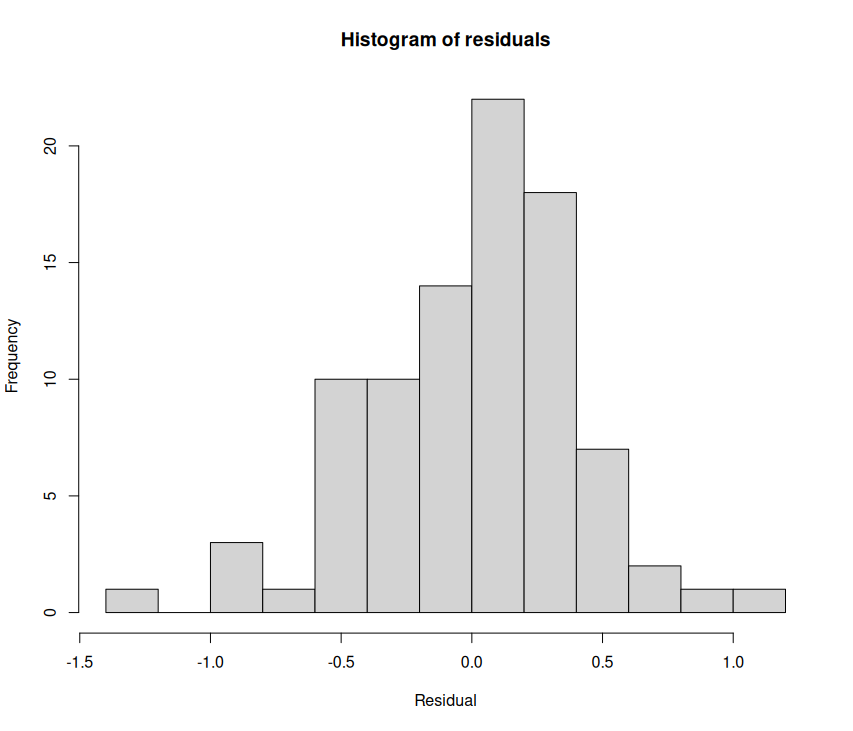
\includegraphics[width=0.8\textwidth]{residuals.png}
    \end{center}
    \caption{The distribution of residuals from the linear model.}
    \label{fig:residuals}
    \end{figure}



    \section{The constrained model}

    We now impose the conditions $\sum_i \tau_i = \sum_j \beta_j = 0$. To do so, we
    replace $\tau_3 = -\tau_1 - \tau_2$, $\beta_3 = -\beta_1 - \beta_2$, whence our
    new model looks like \[
        \vec{y} = \vec{X}^*\vec{\beta}^* + \vec{\epsilon},
    \] where \[
        \vec{X}_{90\times 5}^* = \begin{bmatrix}
            \vec{1} & \vec{1}  & \vec{0}  & \vec{1}  & \vec{0} \\
            \vec{1} & \vec{1}  & \vec{0}  & \vec{0}  & \vec{1} \\
            \vec{1} & \vec{1}  & \vec{0}  & \vec{-1} & \vec{-1} \\
            \vec{1} & \vec{0}  & \vec{1}  & \vec{1}  & \vec{0} \\
            \vec{1} & \vec{0}  & \vec{1}  & \vec{0}  & \vec{1} \\
            \vec{1} & \vec{0}  & \vec{1}  & \vec{-1} & \vec{-1} \\
            \vec{1} & \vec{-1} & \vec{-1} & \vec{1}  & \vec{0} \\
            \vec{1} & \vec{-1} & \vec{-1} & \vec{0}  & \vec{1} \\
            \vec{1} & \vec{-1} & \vec{-1} & \vec{-1} & \vec{-1}
        \end{bmatrix}, \qquad
        \vec{\beta}_{5\times 1}^* = \begin{bmatrix}
            \mu \\ \tau_1 \\ \tau_2 \\ \beta_1 \\ \beta_2
        \end{bmatrix}, \qquad
        \vec{\epsilon} \sim N(0, \sigma^2 \vec{I}_{90}).
    \] With this, $\vec{X}^*$ has full rank $5$. The group estimates
    $\hat{y}_{ij\cdot}$, hence the residuals, remain \emph{unchanged} from $(*)$. The
    least square estimates of the parameters are \[
        \hat{\vec{\beta}}^* = \begin{bmatrix}
            \hat{\mu} \\ \hat{\tau}_1 \\ \hat{\tau}_2 \\ \hat{\beta}_1 \\
            \hat{\beta}_2
        \end{bmatrix} = \begin{bmatrix}
            2.39633556 \\
            0.45933444 \\
            -0.48533222 \\
            0.29267778 \\
            -0.06300556
        \end{bmatrix}.
    \]


    \section{Estimating linear parametric functions}

    Consider the LPF \[
        \vec{A}\vec{\beta} = \begin{bmatrix}
            \tau_1 - \tau_2 \\
            \tau_1 - \tau_3 \\
            \tau_2 - \tau_3
        \end{bmatrix},
    \] where \[
        \vec{A} = \begin{bmatrix}
            0 & 1 & -1 & 0  & 0 & 0 & 0 \\
            0 & 1 &  0 & -1 & 0 & 0 & 0 \\
            0 & 0 &  1 & -1 & 0 & 0 & 0
        \end{bmatrix}.
    \] Here, we can calculate $\rho = \rank(A) = 2$; the first two rows of $A$ are
    linearly independent, the third is their difference. Importantly, each row of $A$
    belongs to $\col(X^\top)$. For example, the first row of $A$ can be expressed as
    the difference of rows 1 and 31 of $\vec{X}$. Thus, $\vec{A}\vec{\beta}$ has a
    BLUE \[
        \widehat{\vec{A}\vec{\beta}} = \vec{A}\hat{\vec{\beta}} =
        \vec{A}(\vec{X}^\top \vec{X})^- \vec{X}^\top \vec{y}.
    \] We calculate \[
        \vec{A}\hat{\vec{\beta}} = \begin{bmatrix}
            0.9446667 \\
            0.4333367 \\
            -0.5113300
        \end{bmatrix}.
    \]

    \section{Confidence intervals/regions for estimates}

    \begin{figure}[H]
    \begin{center}
        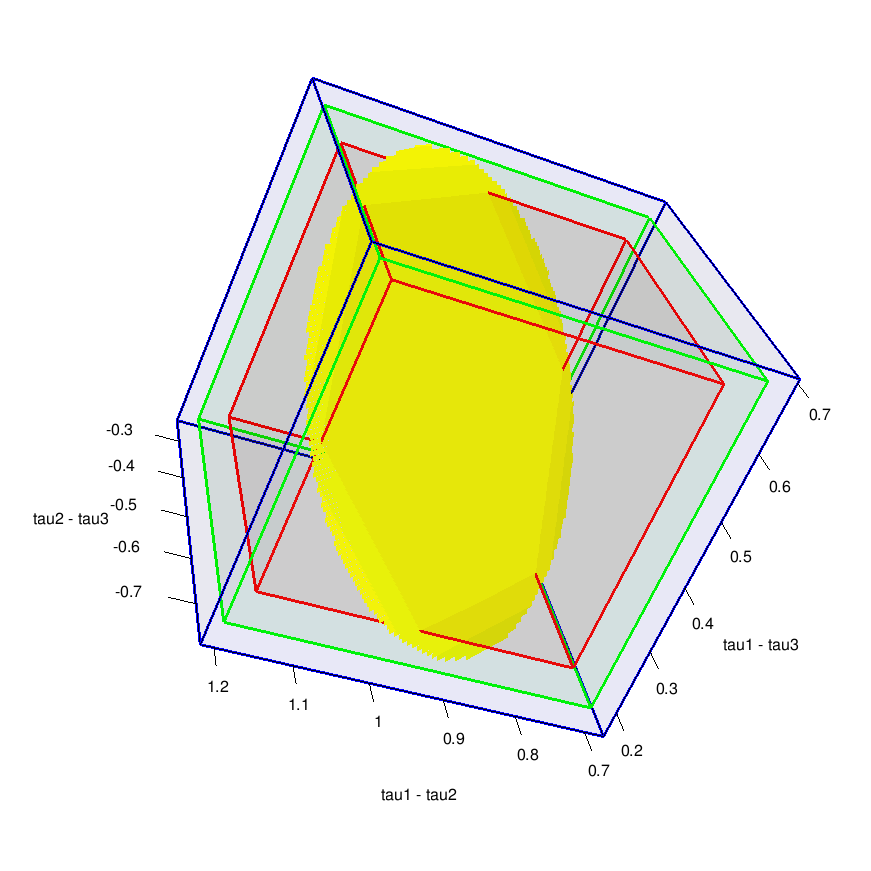
\includegraphics[width=0.8\textwidth]{confidence.png}
    \end{center}
    \caption{
        Confidence regions for $\vec{A}\vec{\beta}$, with $\alpha = 0.05$. The joint
        confidence region is indicated by the \emph{yellow} ellipse, the individual
        confidence intervals are the sides of the \emph{red} cube, the Bonferroni
        confidence region is indicated by the \emph{green} cube, and the Scheff\'e
        confidence region is indicated by the \emph{blue} cube. \\\\
        Note that $(\tau_1 - \tau_2) - (\tau_1 - \tau_3) + (\tau_2 - \tau_3) = 0$.
    }
    \label{fig:confidence}
    \end{figure}


    \subsection{Individual confidence intervals}

    Denoting each row of $\vec{A}$ by $\vec{a}_j^\top$, we can calculate the
    individual $(1 - \alpha)$ confidence intervals for $\vec{a}_j^\top\vec{\beta}$ as
    \[
        \left[
        \vec{a}_j^\top\hat{\vec{\beta}} - \sqrt{\hat{\sigma}^2
        \vec{a}_j^\top(\vec{X}^\top \vec{X})^-\vec{a}_j}\; t_{85; \alpha}, \quad
        \vec{a}_j^\top\hat{\vec{\beta}} + \sqrt{\hat{\sigma}^2
        \vec{a}_j^\top(\vec{X}^\top \vec{X})^-\vec{a}_j}\; t_{85; \alpha}
        \right]
    \] Here, $\hat{\sigma}^2 = R_0^2 / (n - r)$, where $n = 90$, $r = \rank(\vec{X})
    = 5$, and $R_0^2$ is the sum of squares of residuals $\vec{y} - \hat{\vec{y}}$.

    The calculated confidence intervals for $\alpha = 0.05$ are \[
        \tau_1 - \tau_2 : [0.727, 1.162], \qquad
        \tau_1 - \tau_3 : [0.216, 0.651], \qquad
        \tau_2 - \tau_3 : [-0.729, -0.294]
    \] All of them have half-width $0.217$.


    \subsection{Joint confidence region}

    The joint $(1 - \alpha)$ confidence region for $\vec{A}\vec{\beta}$ is given by
    \[
        \{\vec{A}\vec{\beta}\colon (\vec{A}\vec{\beta} -
        \vec{A}\hat{\vec{\beta}})^\top (\vec{A}(\vec{X}^\top\vec{X})^-\vec{A}^\top)^-
        (\vec{A}\vec{\beta} - \vec{A}\hat{\vec{\beta}}) \leq 2\hat{\sigma}^2 F_{2,
        85; 1 - \alpha}, \quad
            \vec{A}\vec{\beta} - \vec{A}\hat{\vec{\beta}} \in
            \col(\vec{A}(\vec{X}^\top\vec{X})^-\vec{A}^\top)
        \}.
    \] It is easy to see that the latter condition is equivalent to the restriction
    that the sum of the first and third components of $\vec{A}\vec{\beta}$ must be
    equal to the second. Thus, this region is a planar section of an ellipsoid, and
    looks like a (filled) ellipse in $\R^3$.

    Indeed, \[
        \vec{A}(\vec{X}^\top\vec{X})^-\vec{A}^\top = \frac{1}{30} \begin{bmatrix}
            2 & 1 & -1 \\
            1 & 2 & 1 \\
            -1 & 1 & 2
        \end{bmatrix}.
    \] 

    \subsection{Bonferroni simultaneous intervals}

    Setting $\gamma = \alpha / \rho$, we have the Bonferroni simultaneous intervals
    \[
        \left[
        \vec{a}_j^\top\hat{\vec{\beta}} - \sqrt{\hat{\sigma}^2
        \vec{a}_j^\top(\vec{X}^\top \vec{X})^-\vec{a}_j}\; t_{85; \gamma}, \quad
        \vec{a}_j^\top\hat{\vec{\beta}} + \sqrt{\hat{\sigma}^2
        \vec{a}_j^\top(\vec{X}^\top \vec{X})^-\vec{a}_j}\; t_{85; \gamma}
        \right]
    \] These together define a cuboidal region in $\R^3$.

    The calculated confidence intervals for $\alpha = 0.05$ are \[
        \tau_1 - \tau_2 : [0.695, 1.194], \qquad
        \tau_1 - \tau_3 : [0.184, 0.683], \qquad
        \tau_2 - \tau_3 : [-0.761, -0.262], \qquad
    \] All of them have half-width $0.250$.


    \subsection{Scheff\'e simultaneous intervals}

    We have the Scheff\'e simultaneous intervals
    \[
        \left[
        \vec{a}_j^\top\hat{\vec{\beta}} - \sqrt{2\hat{\sigma}^2
        \vec{a}_j^\top(\vec{X}^\top \vec{X})^-\vec{a}_j\; F_{2, 85; \alpha}}, \quad
        \vec{a}_j^\top\hat{\vec{\beta}} + \sqrt{\hat{\sigma}^2
        \vec{a}_j^\top(\vec{X}^\top \vec{X})^-\vec{a}_j\; F_{2, 85; \alpha}}
        \right]
    \] These together define a cuboidal region in $\R^3$, larger than the Bonferroni
    intervals and enclosing the ellipsoidal joint confidence region.

    The calculated confidence intervals for $\alpha = 0.05$ are \[
        \tau_1 - \tau_2 : [0.672, 1.217], \qquad
        \tau_1 - \tau_3 : [0.161, 0.706], \qquad
        \tau_2 - \tau_3 : [-0.784, -0.239], \qquad
    \] All of them have half-width $0.273$.
\end{document}
